%%%%%%%%%%%%%%%%%%%%%%%%%%%%%%%%%%%%%%%%%%%%%%%%%%%%%%%%%%%%%%%%%%%%%%%%%%%%%%%%
%% Template de Relatório Parcial baseado nas normas da ABNT voltado 
%% para alunos da UEFS, baseado no modelo de TCC
%% Versão 1.3
%% Desenvolvimento: Danilo de Oliveira Gonçalves
%% Adaptação final: João Carlos Nunes Bittencourt
%% Data: 31/03/2011
%% Atualização: 11/08/2011
%
% TODO: Ajustar o espaçamento do cabeçalho do Apêndice e do Anexo.
%%%%%%%%%%%%%%%%%%%%%%%%%%%%%%%%%%%%%%%%%%%%%%%%%%%%%%%%%%%%%%%%%%%%%%%%%%%%%%%

\documentclass{abnt-uefs} % Classe de formatação da UEFS
\usepackage[utf8]{inputenc}
%\usepackage[T1]{fontenc}
\usepackage[call=authordata,alf,abnt-emphasize=bf,abnt-etal-text=emph,abnt-and-type=&,abnt-etal-list=3,abnt-etal-cite=3,recuo=0.0cm]{abntcite}
\usepackage[brazil]{babel}
\usepackage{mathptmx}
\usepackage{mathtools}
\usepackage[pdftex]{graphicx}
%\usepackage[small,bf]{caption}
\usepackage{longtable}
\usepackage{array}
\usepackage{amssymb,amsmath,amsthm,amsfonts}
%\usepackage{textcomp}
%\usepackage{textcase} 
\usepackage{float} % para as figuras ficarem onde foram colocadas no latex - deve colcoar na figura [H]
\usepackage{color}
%\usepackage{url}

\graphicspath{{./figuras/}} % Diretório padrão de figuras.
%%%%%%%%%%%%%%%%%%%%%%%%%%%%%%%%%%%%%%%%%%%%%%%%%%%%%%%%%%%%%%%%%%%%%%%%%%%%%%%
% Este arquivo faz parte do template de Relatório Parcial baseado nas normas da ABNT 
%  voltado para alunos da UEFS
% Desenvolvimento: Danilo de Oliveira Gonçalves
% Adaptação final: João Carlos Nunes Bittencourt
% Data: 31/03/2011
% Atualização: 30/11/2011
% Descrição do arquivo:
%   Esse arquivo apresenta as definições de constantes que formarão a capa e 
%   a folha de rosto. Siga as instruções e modifique de acordo com o que
%   lhe foi orientado.
%%%%%%%%%%%%%%%%%%%%%%%%%%%%%%%%%%%%%%%%%%%%%%%%%%%%%%%%%%%%%%%%%%%%%%%%%%%%%%%

% ---------- Preambulo ----------
\instituicao{Universidade Estadual de Feira de Santana} % nome da instituicao
\departamento{Colegiado do curso de Engenharia de Computação}
\graduacao{Bacharelado em Engenharia de Computação} % nome do curso
\curso{Engenharia de Computação}

\documento{Trabalho de Conclusão de Curso} % tipo de documento
\titulacao{Bacharel} % [Bacharel]

\titulo{IMPLEMENTAÇÃO DE ALGORITMO PARA CÁLCULO DE SIMILARIDADE MOLECULAR NO SISTEMA NATPRODB} % titulo do trabalho em portugues
\subtitulo{} % caso necessário um sub-título, utilize este campo
\title{Title in English} % titulo do trabalho em ingles

\autor{ANDERSON SOUZA ROCHA} % autor do trabalho
\cita{ROCHA, ANDERSON} % sobrenome (maiusculas), nome do autor do trabalho

\palavraschave{Similaridade Molecular. Banco de Dados Moleculares. Química Computacional.} % palavras-chave do trabalho, separados por ponto
\keywords{Molecular Similarity. Molecular Databases. Computational Chemistry.} % palavras-chave do trabalho em ingles, separados por ponto

\comentario{\UEFSdocumentodata\ apresentado ao \UEFSdepartamentodata\ como requisito parcial para obtenção do grau de \UEFStitulacaodata\ em \UEFScursodata\ pela \ABNTinstituicaodata.}

\orientador{Prof. Dr. Ângelo Amâncio Duarte} % nome do orientador do trabalho
%\orientador[Orientadora:]{Nome da Orientadora} % <- no caso de orientadora, usar esta sintaxe
\coorientador{Prof. Dr. Manoelito C. dos Santos Jr.} % nome do co-orientador do trabalho, caso exista
%\coorientador[Co-orientadora:]{Nome da Co-orientadora} % <- no caso de co-orientadora, usar esta sintaxe

\local{Feira de Santana} % cidade
\data{2016} % ano



 % Elementos da capa
\begin{document}
    \pagestyle{empty}
    \DeclareGraphicsExtensions{.jpg,.pdf,.mps,.png,.bmp,.eps}
    \capa % geração automática da capa
    \folhaderosto % geração automática da folha de rosto
    
   % %%%%%%%%%%%%%%%%%%%%%%%%%%%%%%%%%%%%%%%%%%%%%%%%%%%%%%%%%%%%%%%%%%%%%%%%%%%%%%%
%% Este arquivo faz parte do template de TCC baseado nas normas da ABNT 
%%  voltado para alunos da UEFS
%% Desenvolvimento: Danilo de Oliveira Gonçalves
%% Adaptação final: João Carlos Nunes Bittencourt
%% Data: 31/03/2011
%%%%%%%%%%%%%%%%%%%%%%%%%%%%%%%%%%%%%%%%%%%%%%%%%%%%%%%%%%%%%%%%%%%%%%%%%%%%%%%


% dedicatória (opcional)
\begin{dedicatoria}
Texto da dedicatória.Texto da dedicatória.Texto da dedicatória.Texto da dedicatória.Texto da dedicatória.Texto da dedicatória.Texto da dedicatória.Texto da dedicatória.Texto da dedicatória.
\end{dedicatoria}

%\vfill

%\begin{flushright}
%\hfill \textit{Dedico esta monografia a minha família,\\pelo apoio fornecido e aos meus amigos.\\}
%\end{flushright}

%\vspace*{1cm}

%\clearpage 

   % %%%%%%%%%%%%%%%%%%%%%%%%%%%%%%%%%%%%%%%%%%%%%%%%%%%%%%%%%%%%%%%%%%%%%%%%%%%%%%%
%% Este arquivo faz parte do template de TCC baseado nas normas da ABNT 
%%  voltado para alunos da UEFS
%% Desenvolvimento: Danilo de Oliveira Gonçalves
%% Adaptação final: João Carlos Nunes Bittencourt
%% Data: 31/03/2011
%%%%%%%%%%%%%%%%%%%%%%%%%%%%%%%%%%%%%%%%%%%%%%%%%%%%%%%%%%%%%%%%%%%%%%%%%%%%%%%

% agradecimentos (opcional)
\begin{agradecimentos}
Texto dos agradecimentos.
\end{agradecimentos}

    \begin{resumo}
O processo de desenvolvimento de um fármaco é realizado em diversas etapas, que vão desde
o projeto e estudo de um possível composto farmacofórico até sua sintetização. Grande parte
dos esforços empregados para o desenvolvimento de um novo medicamento são realizados de
forma assistida em computadores. As ferramentas computacionais permitem aos pesquisadores
tanto catalogar de forma mais eficiente suas estruturas de estudo, quanto avaliar de forma mais rápida características estruturais, bioquímicas, e o comportamento de moléculas ao sofrer variações estruturais. Além disso, algumas dessas ferramentas também realizam triagem em bancos de dados moleculares baseados no conceito de similaridade molecular, que é um conceito chave no qual se baseiam grande parte dos esforços dirigidos ao projeto de um novo fármaco. O presente trabalho descreve a adaptação de um algoritmo apropriado para
computação de similaridade molecular em um software desenvolvido para catalogação de
moléculas em banco de dados, visando possibilitar ao pesquisador procurar em sua própria
base de dados, estruturas similares a moléculas de seu interesse de estudo. Um diferencial deste trabalho é que essa ferramenta será disponibilizada livremente para qualquer usuário, e devido às características inerentes à sua implementação, em contrapartida à outras ferramentas
disponíveis para o mesmo fim, este software não necessitará de muitos recursos de hardware
para sua execução, ou seja, é compatível com computadores comuns, e também com qualquer
sistema operacional utilizado pelo pesquisador. De forma resumida, o sistema se comporta da
seguinte forma: Uma vez cadastradas as moléculas e seus respectivos SMILES no banco de dados do usuário, o
pesquisador poderá consultar em seu banco se há ocorrência de estruturas com um grau de
similaridade desejado à molécula inserida para consulta. O sistema converte os SMILES da molécula de
entrada, e das presentes no banco em fingerprints para aplicação da métrica de Tversky para
obtenção de um coeficiente de similaridade, retornando por fim para o pesquisador todas as
moléculas do seu banco que possuem um grau de similaridade igual ou superior ao desejado
(em relação à molécula de entrada). O algoritmo adotado para computação de similaridade molecular foi testado através de uma adaptação do conceito de matriz de confusão e teve como entrada 7 moléculas já disponibilizadas como fármacos, e para os testes realizados no sistema foram verificados que a classificação de moléculas com coeficiente de similaridades $\geq$ 0,8 no sistema se aproximou do comportamento de uma classificação ideal.
\end{resumo}	

    \begin{abstract}
The developing process of a medicine has many stages. Since the project
and study of a possible pharmacophore compound until its synthesizing. Most efforts on the
development of a new medicine are aided by computers. The
computational tools allow the researchers both cataloguing in a more efficient way their study
structures and evaluate in a faster way biochemical, structural features, and the
molecules behavior during structural variations.Moreover, some of these tools also helps in the search for similar structures, that is a key concept in which most efforts towards to develop a new medicine are based.
This work describes the adaptation of appropriate algorithms for computing molecular
similarities in a software developed for molecules tabulation in a database enabling the researcher to screen similar structures to the ones that are in his study concerns at his own database. A differential in this work lies in the fact that this tool is made freely available to any user, and due the inner characteristics of its implementation, face to others tools that exist with the same purpose, this software does not need much hardware resources to run, in other words, it is compatible with common computers, and any operational system used by the researcher. In resume, the system works according to these steps: once the molecules are registered in the user database, the researcher is able to verify in his base if there are structures with a desired degree of similarity to the molecule queried. So, the system converts the inserted molecule, and those ones in the database in fingerprints format in order to use the Tversky's metrics obtaining a table of similarity, and finally retrieving to the researcher all molecules in his database whose similarity coefficient  it is equal or superior to the one desired (regarded to the queried molecule). 
\end{abstract}

    \listadefiguras % geracao automatica da lista de figuras
    \listadetabelas % geracao automatica da lista de tabelas
  %  \listadesimbolos % geracao automatica da lista de símbolos
    \listadesiglas % % geracao automatica da lista de siglas
    % sumario
    \sumario % geracao automatica do sumario
    %---------- Primeiro Capitulo ----------
\chapter{Introdu\c{c}\~ao}
O processo de desenvolvimento de um novo fármaco envolve diversas etapas que englobam desde a pesquisa de um determinado alvo biológico, até a descoberta de compostos com atividades biológicas desejadas e com potencial para se tornarem medicamentos a serem comercializados. Durante esse processo, inúmeras ferramentas e abordagens computacionais podem ser aplicadas visando auxiliar o pesquisador no estudo dos compostos, e também acelerar o desenvolvimento do fármaco. Nos últimos anos, devido a introdução de abordagens computacionais, principalmente nas fases inicias do processo de desenvolvimento de um fármaco, onde o foco do pesquisador é o estudo de um determinado alvo biológico,  tem difundido técnicas de desenvolvimento baseadas no ligante (Ex: Similaridade molecular, modelo farmacofórico) possibilitado assim a identificação de moléculas protótipos para ensaios biológicos \cite{rodrigues2012}. Dentre essas técnicas baseadas no ligante, um conceito já popularizado na comunidade científica é o conceito de similaridade molecular, o qual preconiza que, moléculas que possuem estruturas similares, provavelmente compartilhem propriedades físico-químicas, e atividades biológicas semelhantes \cite{singh2004reasoning}. Dessa maneira, o princípio do processo de desenvolvimento de um fármaco resume-se ao estudo de um determinado alvo biológico para o desenvolvimento de um composto ligante capaz de interagir com o alvo obtendo uma atividade biológica desejada, e em alguns casos realizar uma triagem em bancos de dados moleculares buscando por compostos similares ao ligante em questão (Virtual Screening).

Nessa perspectiva, os esforços para o desenvolvimento e sintetização de um composto ligante podem ser realizados através de sistemas computacionais que aplicam o conceito de similaridade molecular em três grandes eixos segundo \citeonline{kubinyi2008virtual}: a) Exploração computacional e bioquímica de moléculas com estruturas conhecidas (sintetizadas ou não); b) Desenvolvimento de modelos computacionais para estudo de como variações na estrutura molecular afetam a atividade molecular ou as propriedades da molécula; c) Exame de bancos de dados moleculares visando obtenção de um composto similar à estrutura do ligante projetado pelo pesquisador. 

Algumas ferramentas já tem auxiliado pesquisadores nesse sentido como por exemplo o ZINC \cite{irwin2005zinc} e PUBCHEM \cite{li2010pubchem}, ambas ferramentas web que disponibilizam bancos de dados com uma diversidade de moléculas, e também implementam algoritmos para computação de similaridade molecular, permitindo ao pesquisador realizar uma triagem em suas bases de dados a procura de um composto com determinado grau de similaridade a uma determinada estrutura molecular de interesse. Apesar dessas ferramentas auxiliarem pesquisadores a realizarem seus estudos, ainda sofrem de limitação de representação do espaço químico, onde apesar do grande número de moléculas já catalogadas em seus bancos de dados moleculares, o usuário tem seu universo de pesquisa limitado às estruturas disponíveis nesses bancos de dados. Outro problema relacionado a utilização dessas ferramentas já disponíveis é que nenhuma delas fornece ao pesquisador a possibilidade de criação de base de dados com moléculas de sua propriedade, e em alguns casos o usuário acaba disponibilizando suas estruturas em bancos colaborativos para que possam utilizar essas ferramentas para desenvolvimento de suas pesquisas, correndo riscos inclusive de perda de seus direitos autorais sobre os  seus compostos.

Neste trabalho será descrita a implementação de um algoritmo para  realização de triagem virtual baseada no conceito de similaridade molecular no sistema de banco de dados de moléculas, oriundas de fontes naturais endêmicas do bioma semiárido, denominado Natural Products Data Bank (\sigla{NatProDB}{Natural Products Data Bank}), de domínio público, para utilização em modo local (não conectado à Internet), visando: 1) Facilitar a usuários não especialistas em computação, a catalogação de moléculas e manutenção de bancos de dados moleculares, sem a necessidade de uso de bases de dados na Internet; 2) Prover mecanismos para cálculo de similaridade entre moléculas de interesse frente as moléculas depositadas no banco. A computação de similaridade implementada neste sistema é realizada através da métrica de Tversky (coeficiente de similaridade), aplicada sobre a representação computacional de moléculas através de \textit{fingerprints}. A implementação deste método é realizada por uma biblioteca livre denominada Indigo toolkit, que realiza manipulação de moléculas e sub-estruturas \cite{pavlov2011indigo}. Para os testes foi criado um banco de dados para o sistema com um conjunto de moléculas de um banco colaborativo disponibilizado pelo ZINC, e foram enxertadas nesse banco moléculas com grau de similaridade superior a 80\% a um conjunto de moléculas de entrada já testados e utilizados pela indústria farmacêutica. A avaliação do sistema foi realizada verificando os resultados obtidos pelo NatProDB, e avaliando através de matrizes de confusão a capacidade do sistema de classificar corretamente as moléculas 0.8 ou 80\% similares ou não. Os resultados destes testes, assim como os detalhes da implementação deste sistema, serão detalhados nas próximas seções deste trabalho.


                  

\section{Objetivos}

\subsection{Objetivo Geral}

Implementar algoritmo para permitir o processo de triagem virtual de moléculas baseado no conceito de similaridade molecular no sistema NatProDb

\subsection{Objetivos Espec\'ificos}

\begin{itemize}
	\item Implementar um algoritmo para cálculo de similaridade no sistema NatProDB.
	\item Avaliar a eficiência da métrica de similaridade 2D no NatProDB
\end{itemize}



    
\chapter{Fundamentação Teórica}
\label{chap:fundam}
Neste capítulo será discutido na seção 2.1, algumas das ferramentas que já se propõe a realizar
a comparação de moléculas, assim como alguns dos algoritmos que podem ser utilizados na 
análise de similaridade molecular que serão apresentados na seção 2.3, sendo que parte desses 
algoritmos já estão adaptados em algumas das ferramentas a serem apresentadas.
Também será exposto na seção 2.2 algumas formas de representação de uma molécula em um 
ambiente computacional, e sua importância para escolha de qual método de comparação de 
moléculas deverá ser utilizado.
\newpage
\section{FERRAMENTAS PARA COMPUTAÇÃO DE SIMILARIDADE MOLECULAR}
\setcounter{equation}{1}
Devido a importância das ferramentas computacionais no processo de descobertas de fármacos, há diversos esforços dedicados ao desenvolvimento destas ferramentas, tornando-as cada vez mais eficientes e eficazes. Como resultado desses esforços, já se encontram disponíveis alguns sistemas computacionais que aplicam algoritmos de similaridade, realizam busca em bancos de dados, predição de propriedades físico-químicas e atividades biológicas, entre outras diversas funcionalidades importantes na pesquisa e desenvolvimento de fármacos. Esses softwares diferenciam-se de acordo com o custo de sua licença, funcionalidades implementadas, formatos de moléculas aceitos, representação computacional da molécula, método de computação de similaridade molecular, entre outros aspectos.

Uma das ferramentas populares entre pesquisadores na área de química medicinal é o ZINC. O sistema web ZINC é uma ferramenta livre que fornece para o usuário um banco de dados com mais de 21 milhões de estruturas catalogadas \cite{irwin2005zinc}. Além disso, o sistema armazena diversas informações  sobre cada molécula como : massa molecular, centros quirais, coeficiente de partição água-etanol calculado (cLogP). O ZINC armazena estruturas em formatos 2D, tal como o formato Simplified Molecular Input Line Entry System (SMILES), que são representações lineares utilizando uma sequência de caracteres para representação da estrutura molecular \cite{kumar2012}. Além do formato SMILES, o ZINC também aceita como formatos de entradas, Structure Data Format (SDF) e MOL2. O ZINC implementa rotinas para triagem virtual em sua base de dados utilizando os conceitos de similaridade molecular, permitindo ao pesquisador selecionar o grau de similaridade mínimo desejado, e retornando todas as moléculas em seu catálogo (banco de dados) com grau de similaridade igual ou superior ao selecionado pelo usuário \cite{irwin2005zinc}.

Outra ferramenta que pode ser utilizada para a comparação de similaridade entre moléculas é o software ANACONDA. Tal sistema realiza a computação da similaridade entre duas moléculas através da comparação de propriedades de suas respectivas superfícies moleculares utilizando projeção gnomônica . O emprego deste método permite	 a comparação de forma interativa de dois componentes, podendo sugerir modos de superposição entre as moléculas, e assim uma possível geração de um modelo famacofórico \cite{devillers1996}. Esta ferramenta apesar de apresentar bons resultados na comparação de similaridade molecular, não permite a comparação de mais de duas moléculas por consulta, e além disso também não fornece ao pesquisador nenhuma ferramenta para construção, ou manipulação de um banco de dados para catalogação das suas moléculas de estudo, exigindo assim um esforço para o mesmo catalogar suas moléculas de interesse, e realizar uma computação praticamente serial de similaridade entre moléculas que deseja-se estudar 

Utilizando uma abordagem para computação de similaridade molecular baseada na comparação de campos elestrostáticos e de campos de volume esférico, \cite{mestres1997mimic} descrevem um software denominado MIMIC, que implementa rotinas para realização de triagem virtual baseada na comparação de similaridade molecular. Este software permite ao pesquisador obter um índice de similaridade de alta precisão, pois consegue levar em consideração, além da estrutura da molécula, a contribuição de cada átomo na computação da similaridade molecular. Assim como descrito por \cite{devillers1996}, o MIMIC não realiza manipulação de banco de dados, por tanto necessita que o pesquisador insira as moléculas que deseja comparar na entrada do sistema de forma serial. Dessa maneira, para criar um banco de dados para catalogo de moléculas, o usuário necessita utilizar uma outra ferramenta para manipular bancos de dados, o que nem sempre é conveniente para um pesquisador que possua muitas moléculas para estudo, e que por muitas vezes não possui conhecimentos avançados de computação para fazer tal catalogação por conta própria.

Os esforços para implementação de ferramentas computacionais para cálculo de similaridade molecular não se restringem a programas de computador e/ou web sites. Alguns pesquisadores já tem desenvolvido bibliotecas multi-plataformas, capazes de interagir com várias linguagens de programação, e que implementam não somente rotinas para manipulação de moléculas em geral, mas também implementam algoritmos para computação de similaridade molecular. Nessa perspectiva, a Indigo Toolkit surge como uma das bibliotecas de acesso livre mais completas. Desenvolvida pela GGASoftware, e atualmente mantida pelo epam lifescience, Esta ferramenta é capaz de manipular os principais formatos disponíveis para representação de moléculas como: SMILES, SDF, Molfile, entre outros \cite{pavlov2011indigo}. O conjunto de ferramentas disponibilizado por essa biblioteca, permite ao usuário manipular moléculas, computar similaridade, buscar sub-estruturas e reações. A API indigo é capaz de utilizar diversos tipos de descritores moleculares, desde SMILES, até fingerprints (sequência de bits que representa presença ou ausência de uma determinada característica estrututral) e comparando moléculas através de diversas métricas como: coeficiente de Tanimoto, métrica euclidiana, e métrica de Tversky. Para sua utilização é necessário que esta biblioteca seja incorporada a um programa, que pode ser escrito em C/C++, java ou python. Esta biblioteca é utilizada na implementação do NatProDB, conforme será discutido posteriormente.

Utilizando uma abordagem de busca farmacofórica, O Pharmer é considerada uma ferramenta bastante robusta, e já tem sido utilizada até mesmo pelo Zinc no processo de triagem de moléculas similares em seu banco de dados \cite{koes2011pharmer}. O grande diferencial dessa ferramenta é a velocidade de processamento e computação de similaridade molecular em grandes bases de dados, chegando a ser uma ordem de magnitude mais rápido que as ferramentas computacionais já existentes \cite{koes2011pharmer}. O motivo para tal desempenho reside no fato de que em detrimento das demais ferramentas para triagem em bancos de dados moleculares através de modelos famacofóricos (que normalmente realizam a comparação serial de todas as moléculas de sua base de dados), o Pharmer utiliza uma estrutura de organização dados adaptada, denominada Pharmer KDB-tree data structure, e implementa um método de compração baseado em técnicas de computação visual: hashing geométrico e transformada generalizada de Hough. Através da utilização de tais tecnicas, o sistema não somente reduz o custo computacional para comparação de moléculas (grau de similaridade de modelos farmacofóricos), mas também reduz o tempo necessário para consulta no banco uma vez que a estrutura organizacional dos dados em sua base permite um direcionamento do sistema para alvos com maior probabilidade de serem similares.

Outra ferramenta pública que também implementa filtros baseados no conceito de similaridade molecular para triagem virtual de moléculas em bancos de dados (\textit{Virtual Screening})   é o Pubchem \cite{li2010pubchem}. Este sistema possui mais de 25 milhões de estruturas catalogadas em seu banco de dados, e é mantido pelo \textit{National Center for Biotechnology Information} (NCBI). O Pubchem é um dos sistemas bastantes difundidos na comunidade acadêmica devido ao fato de aceitar moléculas sob diversos formatos como (SDF, Mol, SMILES). Além disso, assim como o ZINC \cite{irwin2005zinc} por se tratar de uma fonte de pesquisa pública e de acesso via web, pesquisadores podem utilizar seus recursos computacionais independente de sua localização geográfica, auxiliando pesquisadores em diversos lugares no processo de desenvolvimento de ferramentas para modular processos biológicos e também na identificação de compostos com probabilidade de se tornarem medicamentos utilizados em tratamentos de doenças.   

\section{DESCRITORES MOLECULARES}
O descritor molecular pode ser considerado como o resultado da aplicação de procedimentos lógicos e matemáticos que transformam uma representação química codificada, em uma representação simbólica de uma molécula, em um formato padrão ou resultado de algum experimento padronizado, de forma a facilitar a manipulação dessas estruturas \cite{todeschini2008handbook}. Para o presente trabalho, o descritor molecular consiste no formato sobre o qual uma molécula é representada computacionalmente, e tal formato é importante para a computação de
similaridade, pois o descritor molecular é considerado um fator determinante da métrica a ser
aplicada para cálculo da similaridade estrutural. Nesta seção será apresentado alguns
descritores utilizados por sistemas que calculam similaridade entre moléculas\apud{todeschini2008handbook}{koes2011pharmer}.

\subsection{FingerPrints}
As Fingerprints podem ser consideradas como um descritor molecular complexo. Nesta forma representação computacional de uma molécula, todas as características e grupos funcionais presentes em um dado composto, são codificados em \textit{bitstreams} (Sequencia de bits 0 e 1) únicos para cada estrutura \cite{xue2000molecular}. Além dos grupos funcionais, e características inerentes a uma determinada molécula, as fringerprints também são capazes de armazenar em sua estrutura as distancias entre estruturas do composto, caminhos conexos dessa através de toda a estrutura molecular, ou diferentes tipos de farmacóforos de interesse do pesquisador \cite{todeschini2008handbook}.

Uma das vantagens na utilização de fingerprints na química computacional, é a capacidade de armazenamento de características intrísecas de um composto em um formato de relativamente fácil manipulação por sistemas computacionais. Por exemplo, dentre os modelos de fingerprints mais utilizados na química-computacional, podemos citar a Daylight fingerprint, que utiliza em torno de 2048 bits para armazenamento de propriedades, características, e distâncias moleculares de um único composto, sendo que para esse tipo de descritor não ocorre uma relação direta entre um bit e um determinado grupo funcional/característica (como em modelos de figerprints mais simples), na verdade determinadas caracteristicas, distancias, e/ou propriedades podem ser mapeadas através de algorítmos de \textit{Hashing} para fornecer assim padões de bits cada vez mais específicos, permitindo maior fidelidade na representação das propriedades de uma molécula em um sistema computacional \cite{xue2000molecular}.

Outra importante vantagem da utilização de figerprints para representação computacional de uma molécula reside na simplicidade de aplicação de métodos e métricas para comparacação moléculas baseado no conceito de similaridade molecular \cite{xue2000molecular}. Nesta perspectiva, devido as características intrísicas  desse descritor molecular, o processo de triagem virtual em um banco de dados molecular, pode ser realizado através da geração de fingerprints para cada uma das moléculas do banco e da molécula de consulta, e da aplicação de métricas de similaridade molecular de relativamente fácil implementação em sistemas computacionais como: Coeficiente de Tanimoto, Coeficiente de Tversky, Dice entre outras, que basicamente obtem um determinado coeficiente de similaridade entre duas estruturas moleculares através da realização de um cálculo estatístico que leva em consideração as estruturas e caracteristicas compartilhadas e as singulares das moléculas comparadas. No sistema NatProDB, as fingerprints possuem um papel fundamental no processo de triagem de moleculas de seu banco de dados, uma vez que tal descritor é utilizado para comparação de moléculas conforme será descrito mais aprofundadamente no próximo capítulo.  
     

\subsection{Descritores Farmacofóricos 3D}
Os descritores farmacofóricos tridimensionais quantificam propriedades e as distâncias entre  farmacóforos biológicos importantes para a interação entre o ligante e receptor  \cite{bajorath2004chemoinformatics}. Dentre essas propriedades de interesse de pesquisadores podemos citar: grupos funcionais ou características chaves em determinada orientação, doadores/receptores de ligações de hidrogênio, partes de uma molécula, entre outras. Normalmente, um descritor farmacofórico 3D são compostos basicamente por 3 ou 4 características, e de 3 a 6 distancias entre elas. 
Quando a conformação biológica entre o ligante e receptor é conhecida, é possível identificar     
que características/grupos funcionais são cruciais para ocorrencia dessa ligação. Caso contrário, através de técnicas de triagem virtual (\textit{virtual screening}) pesquisadores podem identificar moléculas que contenham esses grupos funcionais/caracteristicas, ou até mesmo projetar um descritor farmacofórico 3D \cite{bajorath2004chemoinformatics}. 
A aplicação de ferramentas computacionais na comparação de moléculas representadas como descritores farmacofóricos 3D pode ser realizada através do conceito de similaridade molecular aplicando uma transformação nesse descritor em uma \textit{figerprint} (Sequência de bits única para uma molécula), onde bits definidos como '1' simbolizam a presença de uma determinada caracteristica ou grupo funcional, e bits definidos como '0' a ausência de tal estrutura na molécula. Sendo assim, ferramentas computacionais podem calcular a similaridade entre duas moléculas gerando figerprints para cada um dos descritores farmacofóricos 3D e aplicando alguma das métricas já conhecidas para calculo de similaridade entre figerprints, como por exemplo coeficiente de Tanimoto, e coeficiente de Tversky, ambos serão descritos com maiores detalhes em sessões posteriores.          

\subsection{SMILES (Simplified Molecular-Input Line-Entry System)}
     
O SMILES surgiu como descritor molecular para resolver não somente o problema de 
armazenamento de estruturas moleculares em um computador, mas também facilitar a 
manipulação dessas estruturas moleculares por softwares, e também facilitar buscas por 
estruturas moleculares em base de dados na internet internet \cite{kumar2012}. Ainda segundo \cite{kumar2012} é demonstrado que pode-se considerar o SMILE como uma linguagem que permite ao pesquisador representar uma molécula através de uma notação linear padronizada, que muito 
se assemelha à notação utilizada comumente na literatura.

Em uma representação de molécula em formato de SMILES cada átomo é representado por seu símbolo atômico, onde os hidrogênios são omitidos \cite{anderson1987smiles}. Os átomos vizinhos, são representados próximos entre si, e em caso de ligação dupla ou tripla, entre os átomos unidos por tais ligações aparecerão respectivamente os símbolos = e \#. É importante salientar também que ramificações são representadas por parêntesis, e os anéis aromáticos pela alocação de dígitos entre os dois átomos que fecham o anel. A figura 2 exemplifica a conversão de uma estrutura tridimensional em uma notação SMILE, e como tal representação se assemelha a forma como a literatura

\begin{figure}[!htb]
	\centering
	\caption[Exemplo de Molécula representada em SMILE]{Exemplo da representação de uma estrutura 3D em SMILES.}
	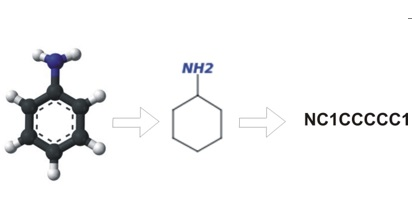
\includegraphics[width=0.5\textwidth]{SMILE.jpg} % <- formatos PNG, JPG e PDF
	\fonte{Autor\nocite{abnTeX2009}}
	\label{fig:dummy}
\end{figure}

O formato do SMILE gerado para a molécula não é necessariamente único, existem
outras representações possíveis, dependendo da estratégia de notação adotada pelo 
pesquisador. Dessa forma é muito comum, para facilitar a busca em bancos de dados, a 
utilização de um formato SMILE canônico, ou seja, que padroniza qualquer SMILE para um 
formato único, o que simplifica a manipulação de qualquer molécula, sem aumentar a 
complexidade dessa operação para o pesquisador (KUMAR, 2012).

Este descritor molecular, além de necessitar de recursos computacionais relativamente 
baixos para representação de uma molécula, devido sua estrutura, é 
bastante utilizado no desenvolvimento de fármacos, principalmente nas atividades que 
envolvem a busca de estruturas similares com uma desejada atividade biológica, pois por ser 
um descritor molecular linear, ele permite a simplificação de uma comparação de moléculas 
realizadas por exemplo em uma forma tridimensional, em uma comparação linear de cadeias 
de caracteres, de mais fácil manipulação em um computador. 

\section{Algorítmos e Métricas para Computação de Similaridade Molecular}

A busca por similaridade molecular é um ponto importante no projeto de um
fármaco pois tal conceito é um dos norteadores para triagem virtual de moléculas de interesse em bancos de dados. Os algorítmos e métricas utilizados na comparação de moléculas baseados no conceito de similaridade são dependentes do descritor molecular utilizado, logo a orientação do método de comparação selecionado deve ser direcionada pela escolha da melhor forma para representar a molécula computacionalmente (TODESCHINI; CONSONNI, 2000). Tal afirmação permite inferir que uma escolha não-adequada de descritor molecular para aplicação de um algoritmo pode inviabilizar a aplicação do mesmo, assim como retornar resultados indesejados, ou não fidedignos com a literatura, prejudicando assim a pesquisa.

\subsection{Coeficiente de Tanimoto}

Existem diversas métricas utilizadas para determinação de similaridade entre duas
moléculas, em geral elas geram um score indicando o grau de similaridade dos compostos comparados. Algumas dessas métricas utilizam distancias euclidianas para determinar esse 
score, como no caso das métricas de Hamming, e Euclidiana. É comum também a utilização 
de coeficientes de associação tais como: Tanimoto, Dice, e coeficientes de cossenos.

O coeficiente de Tanimoto realiza a comparação de moléculas através de uma simples contagem de características compartilhadas (grupos funcionais, propriedades, etc) entre as moléculas submetidas à comparação. Essa contagem gera um determinado valor entre 0 e 1 que indica o grau de similaridade entre as estruturas verificadas \cite{Dogra2007}.

O coeficiente de Tanimoto pode ser utilizado na comparação de descritores moleculares 2D. Nessa perspectiva, este coeficiente se mostra bastante efetivo na comparação de similaridade entre moléculas representadas computacionalmente como \textit{fingerprints}, pois devido a estrutura desse descritor molécular, a comparação de similaridade pode ser realizada através de op
erações booleanas em cadeias binárias para contagem do número de caracteristicas em comum entre cada par de fingerprints \cite{willett2003similarity}. Dessa maneira, a aplicação do coeficiente de Tanimoto para medir similaridade entre duas fingerprints A e B pode ser realizada tomando $N_{A}$ como o número de caracteríticas presentes em A (bits iguais a 1 em A), $N_{B}$ como o número de caracteríticas presentes em B (bits iguais a 1 em B), $N_{AB}$ como o número de caracteríticas compartilhadas por A e B (bits iguais a 1 em A e B), e finalmente o coeficiente de Tanimoto $T_{C}$ pode ser obtido aplicando a equação\eqref{eq:Tanimoto} 

\begin{equation}
T_{C} =\frac{N_{AB}}{N_{A}+N_{B} - N_{AB}}
\label{eq:Tanimoto}
\end{equation}

Nota-se em na equação (\ref{eq:Tanimoto}), que somente são considerados na computação do 
coeficiente de Tanimoto a presença das estruturas (características), a ausência não interfere 
neste processo, o que otimiza a comparação dessas estrutura \cite{Dogra2007}.

\subsubsection{Aplicação do Coeficiente de Tanimoto na Comparação de Fingerprints} 

Seguindo a descrição do coeficiente de Tanimoto apresentada por \cite{Dogra2007}, o trabalho de \cite{machao2011gpu} descreve a utilização dessa métrica para comparação de fingerprints. Em resumo, cada fingerprint presente no banco de dados do autor é representada como vetores de bits com 992 posições, ou seja, para cada molécula são 
verificadas a presença ou ausência de 992 estruturas (características) \cite{Dogra2007}. 

Após verificada essa presença ou ausência dessas estruturas nas moléculas, ou seja gerada a 
fingerprint, é aplicada a equação (\ref{eq:Tanimoto}) sobre as moléculas que se deseja comparar. Assim é obtido o score de similaridade entre as estruturas, e verifica-se se há similaridade ou não entre as moléculas submetidas, conforme podemos observar na  figura (\ref{fig:comparafingerprint}).
\begin{figure}[!htb]
	\centering
	\caption[Cálculo do Coeficiente de Tanimoto sobre duas Fingerprints]{Aplicação do coeficiente de Tanimoto para Computar Similaridade entre Fingerprints.}
	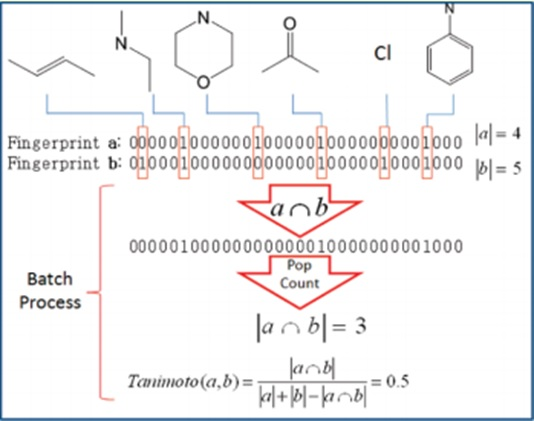
\includegraphics[width=0.5\textwidth]{comparacao_fingerprints.jpg} % <- formatos PNG, JPG e PDF
	\fonte{\cite{machao2011gpu}}
	\label{fig:comparafingerprint}
\end{figure}

Apesar foco central do trabalho apresentado por \cite{machao2011gpu}, não ser a comparação de similaridade molecular, mas sim a paralelização do processo de comparação de similaridade entre bancos de dados moleculares, a figura \ref{fig:comparafingerprint} extraída de sua 
obra, ilustra o procedimento de comparação entre fingerprints, exemplificando desde a 
contagem de estruturas (características) na fingerprint \textit{a} , e na fingerprint \textit{b}, assim como a intersecção entre as características de ambas estruturas ($a\bigcap b$), e por fim a computação do coeficiente de Tanimoto. De acordo com \cite{Dogra2007}, o resultado do coeficiente de Tanimoto (0,5) obtido na figura (\ref{fig:comparafingerprint})  indica baixa similaridade entre as moléculas a e b.

\subsection{Coeficiente de Tversky}
O coeficiente de Tversky pode ser considerado como uma metrica generalizada do coeficiente de Tanimoto \cite{swamidass2007bounds}. Assim como o coeficiente de Tanimoto, o coeficiente de Tversky é uma métrica bastante utilizada para obtenção de índice de similaridade entre moléculas representadas sob descritores moleculares 2D \cite{bajorath2004chemoinformatics}.

Enquanto o coeficiente de Tanimoto calcula a similaridade entre duas moléculas através da taxa de bits comuns (configurados como 1) entre suas respectivas fingerprints   e o número total de bits configurados como 1 em cada molécula como foi observado na figura(\ref{fig:comparafingerprint}), por sua vez o coeficiente de Tversky generaliza a equação (\ref{eq:Tanimoto}) através da introdução dos parametros $\alpha,\beta$:


\begin{equation}
S_{\alpha,\beta}(A,B) =\frac{N_{AB}}{\alpha*N_{A}+\beta*N_{B}+(1-\alpha-\beta)*N_{AB}}
\label{eq:Tversky}
\end{equation}

Conforme podemos observar na equação (\ref{eq:Tversky}),  Quando $\alpha$ = $\beta$ = 1, esta equação se reduz a equação (\ref{eq:Tanimoto}). A introdução desses parâmetros garante ao coeficiente de Tversky uma maior flexibilidade na comparação de similaridade entre duas moléculas uma vez que, os valores de $\alpha$ e $\beta$ permite a aplicação determinadas ponderações na comparação de fingerprints, atribuindo um maior peso a determinadas características presentes na molécula A em detrimento da molécula B, ou vice-versa. Tal característica é importante para buscas de superestruturas e subestruturas de uma molécula, uma vez que um maior peso atribuido a $\alpha$ implica no direcionamento do cálculo de similaridade para superestruturas da molécula A \cite{swamidass2007bounds}. Por outro lado, um maior valor de $\beta$, direciona o cálculo de similaridade para obteção de subestruturas de A, considerando que A é a molécula de entrada no sistema para a qual serão triadas no banco de moléculas as estruturas similares.  

\subsection{LINGO}
O método proposto por \cite{vidal2005lingo} denominado LINGO realiza a computação da similaridade entre moléculas através da conversão dos SMILES de cada molécula (descritor molecular) em um conjunto de substrings sobrepostas de tamanho definido (o autor sugere tamanho 4 para melhores resultados). Desta forma evita-se a manipulação de estruturas tridimensionais, e de grafos, que são mais complexos para se tratar computacionalmente.

Para gerar cada subestrutura do conjunto de substrings a ser utilizado, é necessário a
realização de uma canonização do SMILE, onde converte-se o SMILE de cada molécula para 
uma forma padronizada, conforme já exposto anteriormente. Uma vez canonizadas, as 
SMILES de cada molécula são quebradas em n-(q-1) subestruturas, onde n é o número de 
caracteres do SMILE, e q é o tamanho definido para cada subestrutura. Os conjuntos de 
subestruturas quebradas a partir dos SMILES das moléculas a serem comparadas, são 
agrupados em vetores para aplicação da métrica de similaridade \cite{vidal2005lingo}.

Para computar a similaridade entre os dois vetores (que passaram a representar as 
moléculas), é utilizado o coeficiente de Tanimoto, mas em um formato modificado como podemos verificar na equação \eqref{eq:Modificado}

\begin{equation}
T_{C} =\frac{\sum\limits_{i=1}^{l}1-\frac{|N_{A,i}-N_{B,i}|}{N_{A,i}+N_{B,i}}}{l}
\label{eq:Modificado}
\end{equation}

Observando a equação \eqref{eq:Modificado} verifica-se que $N_{A,i}$ corresponde ao número de ocorrências da i-ésima subestrutura na molécula A (vetor de subestruturas de A), e $N_{B,i}$ o número de 
ocorrências da i-ésima subestrutura na molécula B (vetor de subestruturas de B), e l indica o 
comprimento de um vetor união ($A\bigcup B$). Dessa forma devido ao somatório presente no 
numerador, quanto mais idênticas as frequência de aparições de cada subestrutura em ambas 
moléculas, mais alto será o coeficiente de Tanimoto entre as mesmas, indicando assim uma 
maior similaridade.

\subsection{Localized Co-occurrence Model (LCM)}
Este algoritmo é utilizado para computação de similaridade sobre moléculas
representadas por coordenadas tridimensionais. Segundo \cite{huang2008localized} cada átomo é representado por uma tripla (x,y,z), que informa suas respectivas coordenadas em um espaço tridimensional, e assim para cada átomo, são buscados seus três outros átomos mais próximos, formando um tetraedro denominado Unit Structure, este procedimento é realizado para todos os átomos de uma molécula.

Para cada Unit Structure é calculado o seu volume, e assim então para cada molécula 
será obtido um conjunto de Unit Structures que terá associado as mesmas um valor de 
volume, e então o algoritmo utilizará o menor volume obtido, e o maior volume encontrado 
para definir os limites de um intervalo de volumes para esta molécula. Além disso são 
definidos um conjunto de estados que será associado ao intervalo de volumes, dessa forma o 
intervalo de volumes será particionado de acordo com a quantidade de estados definidos para 
a molécula. Cada Unit Structure recebe um valor de estado correspondente à partição de 
volume que a mesma pertence.

Após definido o estado de cada Unit Structure, para cada par de UnitsStructures o
algoritmo faz uma conexão entre elas caso o centro de massa entre as mesmas seja menor que 
um valor definido, este procedimento é realizado para todos os possíveis pares que podem ser 
formados dentro de um conjunto de Unit Structures. Uma vez formadas todas as conexões 
possíveis, o algoritmo verifica a co-ocorrência das relações das Unit Structuresem relação aos seus valores de estado \cite{huang2008localized}.

Por fim este algoritmo computa a probabilidade de co-ocorrência para cada
combinação de pares de estados, gerando para cada molécula um LCM. A similaridade entre 
duas moléculas é determinada pela comparação dos LCM de cada uma delas, e 
verificando o grau de semelhança entre as representações das moléculas em forma de LCM, 
quanto mais parecidos os LCMs maior a similaridade entre as moléculas, em contrapartida 
quanto menor a semelhança entre os mesmos, menor a similaridade entre as moléculas.





Neste capítulo foram apresentadas algumas das ferramentas utilizadas por pesquisadores
para comparação de moléculas com determinados graus de similaridade. Foi apresentado 
também algumas das principais formas de representação de uma molécula 
computacionalmente (de agora em diante denominada descritores moleculares), e sua 
influência na escolha do algoritmo para computação da similaridade molecular. Além disso 
foi discutido alguns dos algoritmos e métricas possíveis de utilização para realizar tal atividade,contando com uma pequena descrição prévia do selecionado para utilização neste trabalho.No próximo capítulo será discutida as ferramentas utilizadas na adaptação do algoritmo selecionado, bem como a metodologia aplicada para avaliar algoritmo adaptado 
ao sistema NatProDB.



  % %---------- Segundo Capitulo ----------
\chapter{O Sistema NatProDB}
\label{chap:natprodb}

O sistema de gerenciamento de banco de dados molecular (NatProDB) e análise de similaridade molecular proposto é constituído basicamente de dois módulos: 1- Gerenciamento de banco de dados moleculares, e 2- Triagem virtual de moléculas baseado no conceito de similaridade molécular. Para melhor compreensão do sistema, será explanado de forma separada cada um desses módulos. Embora essa metodologia utilizada induza intuitivamente que o sistema é heterogêneo, os módulos citados mais se completam, do que divergem, conforme será verificado em seções posteriores.

\section{Gerenciamento de Bancos de Dados Moleculares}

Uma das principais funcionalidades implementadas no NatProDB é a capacidade de permitir ao pesquisador a criação de sua própria base de dados molecular local, onde o mesmo pode cadastrar, remover, modificar, ou importar arquivos SMI de qualquer estrutura que deseje estudar, armazenando no banco além de propriedades intrísecas de cada molécula, a estrutura molecular do composto através do descritor molecular SMILE. Tal funcionalidade simplifica para o pesquisador o processo de catalogação e gerenciamento de suas moléculas de estudo, além de facilitar a manipulação dessas estruturas para realização de busca por estruturas similares.   
Além de uma ferramenta para catalogação de estruturas, o sistema NatProDb implementa também um filtro para busca de estruturas baseado na regra de Lipinsky \cite{lipinski2012experimental}, que descreve valores limítrofes acerca de características físico-químicas para fármacos com perfil de biodisponibilidade por via oral, a saber: Massa Molecular $\leq$ 500,  \sigla{LopP}{Coeficiente de Partição} $\leq$ 5, \sigla{HBA}{Hydrogen Bond Acceptors} $\leq$ 10, \sigla{HBD}{Hydrogen Bond Donor} $\leq$ 5.

É importante salientar que o sistema NatProDB não realiza a computação dos valores de cada uma das propriedades citadas anteriormente, tais dados são inseridos e/ou importados pelo próprio pesquisador na efetivação de um cadastro de molécula, ou mesmo através de alteração dos dados da mesma.

\section{Triagem Virtual de Moléculas Baseado no Conceito de Similaridade Molécular}

 O sistema NatProDB implementa um algoritmo para triagem de moléculas similares a um molécula de entrada baseada na abordagem descrita na seção 2.2.3, com a ressalva de que ao invés de utilizar o coeficiente de Tanimoto, o sistema utiliza como métrica o coeficiente de Tversky. Para a comparação de estruturas, o sistema armazena as características estruturais da molécula em formato SMILE no seu banco de dados, e ao acessar a rotina de triagem de moléculas por similaridade, o pesquisador pode fornecer  um SMILE de entrada, correspondente a molécula para a qual se procura estruturas similares no banco, e selecionar também o grau de similaridade desejado para busca, variando desde 50-100\%. O sistema por sua vez realiza uma varredura em todo o banco de dados selecionado as moléculas cujo grau de similaridade é igual ou superior ao grau selecionado pelo usuário. Além disso, é possível para o pesquisador aplicar o filtro de Lipinski (Já discutido em seções anteriores), caso as moléculas que ele deseja buscar devam apresentar propriedades específicas que lhes garantem um perfil de biodisponibilidade via oral.

Quando o pesquisador insere uma molécula alvo para realização de uma triagem no banco de dados por moléculas com determinado grau de similaridade, o NatProDB realiza uma chamada a biblioteca indigo toolkit, tal biblioteca realiza duas funções primordiais para computação de similaridade molecular. Primeiramente como exitem diversas formas de gerar um SMILE para uma molécula \cite{kumar2012}, tanto na molécula alvo, como também nas moléculas do banco, é aplicado um algoritmo para canonização de SMILES, para evitar divergencia de resultados devido estruturas representadas sobre diferentes formatações de SMILES. Além disso, a biblioteca indigo toolkit também implementa algoritmos para geração de fingerprints e computação de similaridade molecular baseados no coeficiente de Tversky, ambas funcionalidades são aproveitadas pelo NatProDB para realização da triagem.               

\begin{figure}[!htb]
	\centering
	\caption[Exemplo de uma figura]{Exemplo de uma figura onde aparece uma imagem sem nenhum significado especial.}
	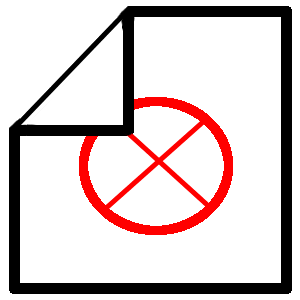
\includegraphics[width=0.2\textwidth]{dummy.png} % <- formatos PNG, JPG e PDF
	\fonte{ABNTEX, 2009\nocite{abnTeX2009}}
	\label{fig:dummy}
\end{figure}

\section{Tabelas}

Tamb\'em \'e apresentado o exemplo da Tabela~\ref{tab:correlacao}, que aparece automaticamente na lista de tabelas. Informa\c{c}\~oes sobre a constru\c{c}\~ao de tabelas no \LaTeX\ podem ser encontradas na literatura especializada~\cite{Lamport1986,Buerger1989,Kopka2003,Mittelbach2004}.

\begin{table}[!htb]
	\centering
	\caption[Exemplo de uma tabela]{Exemplo de uma tabela mostrando a correla\c{c}\~ao entre x e y.}
	\label{tab:correlacao}
	\begin{tabular}{c|c}
		\hline \SPACE
		\textbf{x} & \textbf{y} \\ \hline \SPACE
		1 & 2 \\ \hline \SPACE
		3 & 4 \\ \hline \SPACE
		5 & 6 \\ \hline \SPACE
		7 & 8 \\
		\hline 
	\end{tabular}
	\fonte{Pr\'oprio Autor.}
\end{table}

\section{Equa\c{c}\~oes}

A transformada de Laplace \'e dada na equa\c{c}\~ao~(\ref{eq:laplace}), enquanto a equa\c{c}\~ao apresenta a formula\c{c}\~ao da transformada discreta de Fourier bidimensional\footnote{Deve-se reparar na formata\c{c}\~ao esteticamente perfeita destas equa\c{c}\~oes!}.
\begin{equation}
X(s) = \int\limits_{t = -\infty}^{\infty} x(t) \, \text{e}^{-st} \, dt
\label{eq:laplace}
\end{equation}


\section{Siglas e s\'imbolos}

O pacote abn\TeX\ permite ainda a defini\c{c}\~ao de siglas e s\'imbolos com indexa\c{c}\~ao autom\'atica atrav\'es dos comandos {\ttfamily \textbackslash sigla\{\}\{\}} e {\ttfamily \textbackslash simbolo\{\}\{\}}. Por exemplo, o significado das siglas\sigla{CCECOMP}{Colegiado do Curso de Engenharia de Computa\c{c}\~ao},\sigla{DAEComp}{Diretório Acad\^emico de Engenharia de Computa\c{c}\~ao} e\sigla{UEFS}{Universidade Estadual de Feira de Santana} aparecem automaticamente na lista de siglas, bem como o significado dos s\'imbolos\simbolo{$\lambda$}{comprimento de onda},\simbolo{$v$}{velocidade} e\simbolo{$f$}{frequ\^encia} aparecem automaticamente na lista de s\'imbolos. Mais detalhes sobre o uso destes e outros comandos do abn\TeX\ s\~ao encontrados na sua documenta\c{c}\~ao espec\'ifica~\cite{abnTeX2009}.

    
\chapter{Metodologia}
\label{chap:metodo}
Neste capítulo será apresentado os métodos e ferramentas aplicados no
desenvolvimento e implementação do algoritmo a ser adaptado no NatProDB. Também será
apresentado a metodologia dos testes realizados sobre o algoritmo escolhido para adptação ao
NatProDB.

\section{FERRAMENTAS UTILIZADAS PARA IMPLEMENTAÇÃO}

Tanto o módulo de gerenciamento de banco de dados do sistema NatProDB, assim como o método aplicado para  realização de triagem de moléculas baseado no coeficiente de similaridade molecular foram desenvolvidos baseados no paradigma de Programação Orientada à Objetos (POO), e utilizando como padrão de projeto o \textit{Model View Controller}, visando assim desacoplar o código do sistema, e também facilitar a manutenção e inclusão de novas funcionalidades no mesmo \cite{patterns2003model}. A implementação do sistema, assim como o desenvolvimento do algoritmo de cálculo de similaridade molecular fora realizados utilizando como linguagem de programação Java devido ao fato dessa linguagem de programação ser multi-plataforma (capaz de ser executada em vários sistemas operacionais),  gratuita ,e também por questões de compatibilidade com a biblioteca indigo toolkit e com o próprio módulo de gerenciamento de banco de dados do NatProDB. O ambiente selecionado para o desenvolvimento foi o NetBeans 8.1.

\section{ALGORITMO E MÉTRICA PARA CÁLCULO DE SIMILARIDADE NO NATPRODB}

 Conforme já discutido na seção 2.2, a escolha do descritor molécular a ser utilizado é um ponto chave para decisão sobre que algoritmo/métrica melhor se adequa para comparação de similaridade entre moléculas \cite{todeschini2008handbook}. Nesta perspectiva, o sistema NatProDB utiliza dois descritores moleculares para realizar cálculo de similaridade molecular: SMILES, e Fingerprint. Os SMILES são utilizados para armazenar no banco de dados do sistema a estrutura física das moléculas devido a sua simplicidade na representação da molécula em formato 2D e também baixo custo computacional para armazenamento das caracteristicas estruturais dos compostos. Os SMILES do ligante (estrutura de interesse do pesquisador) e das moléculas presentes no banco de dados do NatProDB são utilizadas na fase de pré-processamento das estruturas, onde as mesmas são preparadas para posterior comparação de similaridade. Nesta fase, devido ao fato de existirem diversos métodos para geração de SMILES para uma molécula \cite{kumar2012}, visando evitar possíveis distorções nos resultados da comparação de similaridade entre as estruturas, tanto o SMILES do ligante quanto os SMILES das moléculas presentes no banco passam por um processamento de canonização, que basicamente re-organiza o SMILES de forma a garantir que todos os SMILES do sistema sejam obtidos seguindo o mesmo padrão de geração \cite{kumar2012}, obtendo assim estruturas únicas para cada uma das moléculas do sistema. Tal canonização é realizada no sistema pela biblioteca Indigo toolkit, que implementa algoritmo para obtenção de SMILES únicos conforme descrito por Pavlov (2011).

Uma vez obtidas os SMILES canônicos das moléculas, o sistema NatProDB realiza uma conversão    
desses SMILES para outro descritor molecular, no caso Fingerprints. Apesar da existência de metodologias de comparação de similaridade baseadas nos SMILES, como por exemplo o LINGO \cite{vidal2005lingo}, as fingerprints se mostram mais populares na literatura para realização de comparação de similaridade entre moléculas \cite{varnek2011fragment}. Primeiramente, devido a forma como a fingerprint codifica a estrutura molecular e as características intrísecas de cada composto como uma sequência de bits '1' e '0' favorece a aplicação de métricas de similaridade já difundidas na comunidade científica como: Coeficiente de Tanimoto, e Coeficiente de Tversky \cite{willett2003similarity}. Além disso, a utilização das Fingerprints para comparação de similaridade molecular, reduz a computação de similaridade entre duas moléculas a contagem e comparação de bits '1' presentes em cada uma das estruturas. Dessa maneira, para realizar  a conversão dos SMILES das moléculas para Fingerprint, o sistema NatProDB utiliza a biblioteca indigo toolkit, que implementa uma rotina para  realizar tal conversão, finalizando assim o pré-processamento das estruturas para aplicação de métrica de similaridade adotada para o sistema.

A partir das fingerprints obtidas no pré-processamento das estruturas, o algorítmo implementado no sistema NatProDB para comparação de similaridade entre moléculas, segue o método descrito nas seção 2.3.1.1. Basicamente, é realizada a contagem de características em comum e distintas entre as fingerprints de entrada (ligante) e as fingerprints das moléculas do banco, e então aplicada uma métrica para obtenção do coeficiente de similaridade. Diferentemente do método descrito na seção 2.3.1.1, ao invés de utilizar o coeficiente de Tanimoto  descrito na equação (\ref{eq:Tanimoto}) como métrica de similaridade para realização da triagem em seu banco de dados, o NatProDB utiliza o coeficiente de Tversky. Tal escolha é orientada pela característica deste coeficiente de permitir o favorecimento das caracterícas presentes na fingerprint de uma moléculas em detrimento da outra através da introdução dos parâmetros $\alpha$ e $\beta$ na equação (\ref{eq:Tversky}). Através do aumento e diminuição dos parametros $\alpha$ e $\beta$, o sistema NatProDB consegue flexibilizar seu método para comparação de similaridade, permitindo assim a comparação não somente de similaridade molecular, mas também a busca de super-estruturas e/ou subestruturas de acordo com os valores selecionados para esses coeficientes. Assim como na etapa de pré-processamento das moléculas, a computação da similaridade entre estruturas através do coeficiente de Tversky é realizado também pela indigo toolkit, que possui uma rotina chamada \textit{similarity}(), que recebe duas fingerprints, e o tipo de coeficiente a ser aplicado (Coeficiente de Tversky para o caso do NatProDB), retornando para o sistema o grau de similaridade entre as duas fingerprints. Este método é aplicado serialmente entre a molécula de entrada (ligante) e cada uma das moléculas cadastrada no banco de dados do sistema, retornando para o pesquisador somente as moléculas cujo coeficiente de Tversky encontrado é superior ao grau de similaridade selecionado previamente pelo pesquisador.  

\section{TESTES}

Para realização dos testes no sistema, foram selecionados 7 moléculas-alvo  com estruturas moleculares diversificadas entre si, (citar moléculas) e que já são distríbuidas para o mercado como fármacos, ou seja substâncias que contem estruturas que possibilitam sua absorção e metabolização pelo corpo humano. Visando criar um banco controlado para os testes, foram baixadas 47770 moléculas de um banco molecular colaborativo disponibilizado pelo ZINC \cite{irwin2005zinc} para o banco local do NatProDB. Para garantir que não exitia moléculas com grau de similaridade superior a 0.8 ou 80\% às moléculas-alvo, foram realizadas consultas nesse banco colaborativo através do ZINC buscando estruturas com grau de similaridade superior a 80\% ou 0.8 para cada uma das moléculas selecionadas para teste. A escolha do coeficiente de similaridade de 0.8 ou 80\% como limiar foi baseada no trabalho de Drogra(2007) que afirma que estruturas com coeficiente de similaridade superior ou igual a 0,85 podem ser consideradas similares. Para cada uma dessas 7 consultas o ZINC não retornou nenhuma molécula 80\% similar ou com grau de similaridade superior às moléculas alvo. Após populado o banco de dados do NatProDB, foram enchertados nesse banco local: 50 moléculas com grau de similaridade $\geq $ 0.8 ou $\geq $80\% ao acetaminophen, 50 moléculas com grau de similaridade $\geq $ 0.8 ou $\geq $80\% à fluoxetina, 50 moléculas com grau de similaridade $\geq $0.8 ou $\geq $80\% ao Glyburide, 50 moléculas com grau de similaridade $\geq $ 0.8 ou $\geq $80\% ao Imatinib, 34 moléculas com grau de similaridade $\geq $ 0.8 ou $\geq $80\% ao Isosorbid, 50 moléculas com grau de similaridade $\geq $0.8 ou $\geq $80\% ao Vinblastine, 50 moléculas com grau de similaridade $\geq $0.8 ou $\geq $80\% ao propanolol. Todas essas estruturas foram extraídas do PUBCHEM \cite{li2010pubchem}, que além de implementar algoritmo para recuperação de moléculas baseado no conceito de similaridade, permite o download dessas estruturas em formato .smi, que é um formato já aceito pelo NatProDB para importação de moléculas.

Após a população do banco de dados do NatProDB foram repetidas no sistema as mesmas 7 consultas realizadas no ZINC, visando assim validar o método implementado para computação de similaridade molecular verificando se o algoritmo aplicado consegue recuperar para cada uma das moléculas-alvo, as moléculas 80\% ou 0.8 similares as mesmas dentro do conjunto de moléculas inseridas no banco, . Os resultados obtidos   
   





   

    \chapter{Resultados e Discussões}
\label{chap:resul}
 
 De acordo com \citeonline{Dogra2007}, a similaridade entre duas moléculas pode ser verificada quando o coeficiente de similaridade resultante da comparação de duas estruturas é superior a 80\%. Desta maneira para o primeiro teste realizado no sistema, tendo como alvo o acetaminophen e utilizando o limiar de similaridade citado anteriormente, das 50 moléculas$\geq $80\% similares (extraídas do PUBCHEM) inseridas no banco do NatProDB, o algoritmo implementado no sistema recuperou corretamente 45 delas com coeficiente de similaridade superior a 80\% (Verdadeiro Positivo $V_P$), 5 delas foram classificadas pelo NatProDB com similaridade inferior a 80\% (Falso Negativo $F_P$), como podemos verificar na tabela \ref{tab:Acetaminophen} 
 
 \begin{table}[!htb]
	\centering
	\footnotesize
	\caption[Classificação de moléculas similares ao Acetaminophen]{Classificação de moléculas similares ao Acetaminophen}
	\label{tab:Acetaminophen}	
	\begin{tabular}{p{4cm}ccc}
		\hline \SPACE
		\textbf{}&\textbf{Similaridade $\geq $ 80\%} & \textbf{Similaridade $\leq $ 80\%} \\ \hline \SPACE
	Moléculas classificadas c/ similaridade $\geq $ 80\%  &	45 & 0 \\ \hline \SPACE
	Moléculas classificadas c/ similaridade $\leq $ 80\%  & 5 & 47742\\ \hline 
	\end{tabular}
	\fonte{Pr\'oprio Autor.}
\end{table}
A partir da matriz de confusão  representada na tabela \ref{tab:Acetaminophen} podemos observar para esse teste uma Acurácia = 99,00\% equação\eqref{eq:Acuracia}, Sensibilidade = 90,00\% equação\ref{eq:Sensibilidade}, Medida F-Score = 94,70\% equação\eqref{eq:FMedida}, Precisão = 100\% equação\eqref{eq:Precisao}, Especificidade = 100\% equação\eqref{eq:Especificidade}

Para o segundo teste realizado, tendo como alvo a fluoxetina, e utilizando o mesmo limiar de similaridade aplicado anteriormente, das 50 moléculas $\geq $80\% similares a fluoxetina enxertada no NatProDB (extraídas do PUBCHEM), o algoritmo implementado no NatProDB recuperou corretamente 48 dessas estruturas ($V_P$), e apenas duas delas foram classificadas com coeficiente de similaridade inferior a 80\%($F_N$), e nenhum $F_P$ foi verificado conforme podemos observar na tabela \ref{tab:Fluoxetina}. 

 \begin{table}[!htb]
	\centering
	\footnotesize
	\caption[Resultado Obtido da Busca de Estruturas $\geq$80\% Similares a Fluoxetina]{Resultado Obtido da Busca de Estruturas $\geq$80\% Similares a Fluoxetina}
	\label{tab:Fluoxetina}	
	\begin{tabular}{p{4cm}ccc}
		\hline \SPACE
		\textbf{}&\textbf{Similaridade $\geq $ 80\%} & \textbf{Similaridade $\leq $ 80\%} \\ \hline \SPACE
	Moléculas classificadas c/ similaridade $\geq $ 80\%  &	48 & 0 \\ \hline \SPACE
	Moléculas classificadas c/ similaridade $\leq $ 80\%  & 2 & 47742\\ \hline 
	\end{tabular}
	\fonte{Pr\'oprio Autor.}
\end{table}       
A partir da tabela \ref{tab:Fluoxetina} também podemos observar que para esse teste foram obtidas: Acurácia = 99,00\% equação\eqref{eq:Acuracia}, Sensibilidade = 96,00\% equação(\ref{eq:Sensibilidade}), Medida F-Score = 97,90\% equação\eqref{eq:FMedida}, Precisão = 100\% equação\eqref{eq:Precisao},  Especificidade = 100\% equação\eqref{eq:Especificidade}.

O terceiro teste realizado teve como alvo Glyburid. Sob o mesmo limiar de similaridade dos testes anteriores, das 50 moléculas $\geq $80\% similares ao Glyburid, inseridas no banco de dados do NatProDB (extraídas do PUBCHEM), o algoritmo implementado  recuperou corretamente todas as 50 estruturas ($V_P$), e por tanto nenhuma delas foram classificadas com coeficiente de similaridade inferior a 80\%($F_N$), o que gerou uma  Acurácia = 100\%  equação\eqref{eq:Acuracia}, Sensibilidade = 100\% equação(\ref{eq:Sensibilidade}), Medida F-Score = 100\% equação\eqref{eq:FMedida}, Precisão = 100\% equação\eqref{eq:Precisao},  Especificidade = 100\% equação\eqref{eq:Especificidade}. conforme podemos observar na tabela \ref{tab:Glyburid}.

 \begin{table}[!htb]
	\centering
	\footnotesize
	\caption[Resultado Obtido da Busca de Estruturas $\geq$ 80\% Similares ao Glyburid]{Resultado Obtido da Busca de Estruturas $\geq$ 80\% Similares ao Glyburid}
	\label{tab:Glyburid}	
	\begin{tabular}{p{4cm}ccc}
		\hline \SPACE
		\textbf{}&\textbf{Similaridade $\geq $ 80\%} & \textbf{Similaridade $\leq $ 0.8} \\ \hline \SPACE
	Moléculas classificadas c/ similaridade $\geq $ 0.8  &	50 & 0 \\ \hline \SPACE
	Moléculas classificadas c/ similaridade $\leq $ 0.8  & 0 & 47742\\ \hline 
	\end{tabular}
	\fonte{Pr\'oprio Autor.}
\end{table} 

O quarto teste realizado teve como alvo a molécula Imatinib. A triagem de moléculas no banco do NatProDB cujo coeficiente de similaridade $\geq$ 80\% com relação a molécula-alvo, retornou 49 das 50 estruturas $\geq$80\% similares ao imatinib enxertadas no banco. Dessa maneira foram obtidos 49  $V_P$, apenas 1 $F_P$, e novamente nenhum $F_N$ foi verificado. A partir desse resultado foram obtidas: Acurácia = 99,00 equação\eqref{eq:Acuracia}, Sensibilidade = 98,00\% equação(\ref{eq:Sensibilidade}), Medida F-Score = 98,90\% \eqref{eq:FMedida}, Precisão = 100,00\% equação\eqref{eq:Precisao},  Especificidade = 100,00\% \eqref{eq:Especificidade}. conforme podemos observar na tabela \ref{tab:Imatinib}

 \begin{table}[!htb]
	\centering
	\footnotesize
	\caption[Resultado Obtido da Busca de Estruturas $\geq$80\% Similares ao Imatinib]{Resultado Obtido da Busca de Estruturas $\geq$80\% Similares ao Imatinib}
	\label{tab:Imatinib}	
	\begin{tabular}{p{4cm}ccc}
		\hline \SPACE
		\textbf{}&\textbf{Similaridade $\geq$80\%} & \textbf{Similaridade $\leq $80\%} \\ \hline \SPACE
	Moléculas classificadas c/ similaridade $\geq $ 80\%  &	50 & 0 \\ \hline \SPACE
	Moléculas classificadas c/ similaridade $\leq $ 80\%  & 0 & 47742\\ \hline 
	\end{tabular}
	\fonte{Pr\'oprio Autor.}
\end{table}

O quinto teste realizado no sistema teve como alvo o Isosorbid. A consulta realizada no banco do NatProDB por estruturas 80\% similares à molécula-alvo, retornou todas as 34 moléculas $\geq$ 80\% similares as que foram enxertadas no banco do sistema, não gerando assim nenhum falso-positivo ou falso-negativo. Consequentemente foram obtidas a partir dos resultados apresentados na tabela \ref{tab:Isosorbid}: Acurácia = 100\% equação\eqref{eq:Acuracia}, Sensibilidade = 100,00\% equação(\ref{eq:Sensibilidade}), Medida F-Score = 100,00\% \eqref{eq:FMedida}, Precisão = 100,00\% equação\eqref{eq:Precisao},  Especificidade = 100,00\% equação\eqref{eq:Especificidade}.

 \begin{table}[!htb]
	\centering
	\footnotesize
	\caption[Resultado Obtido da Busca de Estruturas $\geq$80\%  Similares ao Isosorbid]{Resultado Obtido da Busca de Estruturas $\geq$80\% Similares ao Isosorbid}
	\label{tab:Isosorbid}	
	\begin{tabular}{p{4cm}ccc}
		\hline \SPACE
		\textbf{}&\textbf{Similaridade $\geq $80\%} & \textbf{Similaridade $\leq $80\%} \\ \hline \SPACE
	Moléculas classificadas c/ similaridade $\geq $80\%  &	34 & 0 \\ \hline \SPACE
	Moléculas classificadas c/ similaridade $\leq $80\%  & 0 & 47758\\ \hline 
	\end{tabular}
	\fonte{Pr\'oprio Autor.}
\end{table}

Para o sexto teste foi selecionada como molécula-alvo o Vinblastine. A triagem realizada no banco de dados do NatProDB por estruturas $\geq$ 80\% similares a molécula-alvo, recuperou todas as 50 moléculas $\geq$80\% similares ao Vinblastine enxertadas no banco de dados do sistema. Novamente, assim como no teste anterior, não foi verificada a ocorrência de falsos-positivos e/ou falsos-negativos, resultando em medidas de: Acurácia = 100,00\% equação\eqref{eq:Acuracia}, Sensibilidade = 100,00\% equação(\ref{eq:Sensibilidade}), Medida F-Score = 100,00\% equação\eqref{eq:FMedida}, Precisão = 100,00\% equação\eqref{eq:Precisao},  Especificidade = 100,00\% equação\eqref{eq:Especificidade}. Conforme podemos verificar pela tabela \ref{tab:Vinblastine}

 \begin{table}[!htb]
	\centering
	\footnotesize
	\caption[Resultado Obtido da Busca de Estruturas $\geq$ 80\% Similares ao Vinblastine]{Resultado Obtido da Busca de Estruturas $\geq$80\% Similares ao Vinblastine}
	\label{tab:Vinblastine}	
	\begin{tabular}{p{4cm}ccc}
		\hline \SPACE
		\textbf{}&\textbf{Similaridade $\geq $ 80\%} & \textbf{Similaridade $\leq $ 80\%} \\ \hline \SPACE
	Moléculas classificadas c/ similaridade $\geq $ 80\%  &	50 & 0 \\ \hline \SPACE
	Moléculas classificadas c/ similaridade $\leq $ 80\%  & 0 & 47742\\ \hline 
	\end{tabular}
	\fonte{Pr\'oprio Autor.}
\end{table}

\newpage
O sétimo teste realizado teve como molécula-alvo o Propanolol. A consulta realizada no NatProDB buscando as estruturas $\geq$ 80\% similares ao Propanolol recuperou 42 das 50 moléculas enxertadas no banco do sistema (Verdeiros positivos $V_P$), e as 8 moléculas restantes foram classificadas com coeficiente de similaridade inferior a 0.8 (Falso negativos $F_P$). A partir desse dados foram obtidas a partir da tabela (\ref{tab:Propanolol}): Acurácia = 99,00\% equação\eqref{eq:Acuracia}, Sensibilidade = 84,00\%  equação(\ref{eq:Sensibilidade}), Medida F-Score = 91,00\% equação\eqref{eq:FMedida}, Precisão = 100,00\% equação\eqref{eq:Precisao},  Especificidade = 100,00\% equação\eqref{eq:Especificidade}.  

Os resultados desse teste podem ser verificado na matriz de confusão (\ref{tab:Propanolol})
\begin{table}[!htb]
	\centering
	\footnotesize
	\caption[Resultado Obtido da Busca de Estruturas $\geq$80\% Similares ao Propanolol]{Resultado Obtido da Busca de Estruturas $\geq$80\% Similares ao Propanolol}
	\label{tab:Propanolol}	
	\begin{tabular}{p{4cm}ccc}
		\hline \SPACE
		\textbf{}&\textbf{Similaridade $\geq $ 80\%} & \textbf{Similaridade $\leq $ 80\%} \\ \hline \SPACE
	Moléculas classificadas c/ similaridade $\geq $ 80\%  &	42 & 0 \\ \hline \SPACE
	Moléculas classificadas c/ similaridade $\leq $ 80\%  & 8 & 47742\\ \hline 
	\end{tabular}
	\fonte{Pr\'oprio Autor.}
\end{table}

\begin{table}[!htb]
	\centering
	\footnotesize
	\caption[Resumo dos Resultados Obtidos nos Testes Realizados]{Resumo dos Resultados Obtidos nos Testes Realizados}
	\label{tab:ResumoResultados}	
	\begin{tabular}{|c|c|c|c|c|c|c|}
		\hline \SPACE
		\textbf{Teste}&\textbf{Acurácia}&\textbf{Sensibilidade \%}&\textbf{F-Score \%}&\textbf{Precisão \%}&\textbf{Especificidade \%}&\textbf{FPR \%} \\ \hline \SPACE
	1\textordmasculine &99,00&90,00&94,70&100,00&100,00&0,00 \\ \hline \SPACE
	2\textordmasculine &99,00&96,00&97,90&100,00&100,00&0,00\\ \hline 
	3\textordmasculine &100,00&100,00&100,00&100,00&100,00&0,00\\ \hline
	4\textordmasculine &99,00&98,00&98,90&100,00&100,00&0,00\\ \hline
	5\textordmasculine &100,00&100,00&100,00&100,00&100,00&0,00\\ \hline
	6\textordmasculine &100,00&100,00&100,00&100,00&100,00&0,00\\ \hline
	7\textordmasculine &99,00&84,00&91,00&100,00&100,00&0,00\\ \hline
	\end{tabular}
	\fonte{Pr\'oprio Autor.}
\end{table}
 
De acordo com \citeonline{davis2006relationship}, embora as medidas de acurácia e F-medida forneçam uma medida global da qualidade da classificação, na qual quão mais próximos de 100,00\% os valores obtidos para as mesmas melhor a classificação, o autor relata que uma classificação ideal ocorre quando a Sensibilidade \eqref{eq:Sensibilidade} $\simeq 100,00$\% , e FPR \eqref{eq:FPR}  $\simeq 0$\%. Sob essa perspectiva, tomando como base o pior caso dos testes realizados no sistema, que teve como alvo a molécula de propranolol - que reportou $F_N$ = 8, podemos facilmente identificar a partir tabela de resumo dos testes (\ref{tab:ResumoResultados}) que foram obtidas uma Sensibilidade = 84\%, e FPR = 0\%, o que indica que o método aplicado para separar as moléculas $\geq$ 80\% similares ao propranolol obteve uma resposta satisfatória, uma vez que ambas sensibilidade e FPR se aproximaram respectivamente de 100\% e 0\% (classificador ideal). Estendendo tal verificação para todos os testes realizados, foi observado que não ocorreram $F_P$ nos testes realizados, ou em outras palavras, o método  implementado para triagem virtual de moléculas baseado no conceito 80\% de  similaridade não retornou nenhuma molécula com coeficiente de similaridade inferior a  para cada uma das moléculas-alvo testadas. Consequentemente, as sensibilidades verificadas em todos os testes realizados variam dentro de um intervalo de [84,00\% - 99,00\%], o que de acordo com \citeonline{davis2006relationship}  pode ser considerado como um comportamento próximo de um classificador ideal.




            


   

   
   \chapter{Considerações Finais}
\label{chap:conclusao}

O presente trabalho é fruto de um projeto de iniciação científica desenvolvido em uma parceria entre o Laboratório de Computação de Alto Desempenho(\sigla{LACAD}{Laboratório de Computação de Alto Desempenho}) e o Laboratório de Modelagem Molecular (\sigla{LMM}{Laboratório de Modelagem Molecular}) da UEFS, no qual foi proposto o estudo e implementação de um algoritmo para o sistema NatProDB visando possibilitar ao sistema a realização de uma triagem virtual de moléculas a partir do conceito de similaridade molecular. O sistema desenvolvido neste trabalho  permite aos pesquisadores construírem localmente suas próprias bases de dados, e selecionar dentro do seu banco moléculas similares aos ligantes de seu interesse para realização de estudos. 

A aplicação de uma abordagem de comparação de moléculas 2D proposta neste trabalho simplifica  a computação de similaridade molecular, uma vez que, permite a utilização de descritores moleculares lineares como as fingerprints, e também a aplicação de técnicas de comparação como o Coeficiente de Tversky ou até mesmo o Coeficiente de Tanimoto, que calculam a similaridade entre estruturas através da contagem de características/grupos funcionais presentes em cada molécula. Entretanto, tal modelo sofre de algumas limitações a serem consideradas, como por exemplo: a variação de conformações de uma dada molécula podem gerar coeficientes de similaridade altos somente para determinadas conformações, ou seja, mesmo compartilhando uma estrutura molecular parecida, as moléculas são similares somente para alguns estados conformacionais \cite{rodrigues2012}. Além disso, por se tratar de uma comparação baseada em contagem de características e avaliação estrutural das moléculas, questões como rotações, propriedades intrínsecas de alguns compostos, e até mesmo átomos quirais, não são tratadas pelo algoritmo implementado no sistema, o que pode ocasionar obtenção de índices de similaridade altos entre duas estruturas que não necessariamente possuem atividades biológicas semelhantes. Tais deficiências podem ser solucionadas através da utilização de abordagens híbridas que além da comparação estrutural 2D, consideram propriedades intrínsecas de cada composto obtidas via processamento de descritores 3D, mas que não necessariamente podem ser estendidos  como solução para todos os possíveis casos.

Apesar das limitações citadas anteriormente, o método implementado no NatProDB é uma abordagem bastante difundida na literatura, e já vem sendo utilizada inclusive por sistemas consolidados na comunidade científica como o PubChem por exemplo. Além disso, devido a escassez de ferramentas gratuitas que se proponham a fornecer um ambiente computacional onde o pesquisador possa controlar e gerenciar as suas moléculas, assim como realizar triagem em bancos locais através do conceito de similaridade molecular, o sistema desenvolvido surge como uma ferramenta para auxiliar esses pesquisadores desenvolverem seus estudos e até mesmo criarem  base de dados com estruturas de sua propriedade para posterior publicação.

Embora o sistema NatProDB já venha sendo utilizado por pesquisadores do LMM, esse projeto evoluiu de forma a abarcar não somente o estudo de estruturas moleculares localmente, mas também permitir a difusão das moléculas oriundas do semi-árido baiano para a comunidade científica em geral. Nesse sentido, recentemente foi criado um ambiente web para o NatProDB, que fornece a possibilidade de acesso a um catalogo de moléculas extraídas de fontes naturais endêmicas do oriundas  do bioma semi-árido. Como próximos passos deste projeto, o grupo pretende adaptar o algorítimo implementado no sistema local também na versão web, assim como adaptar métodos de comparação de estruturas em 3D visando assim suprir algumas das deficiências citadas anteriormente.     
     

  
    % Aqui começa a bibliografia da monografia
    \bibliographystyle{abnt-alf}
    \bibliography{abnt-uefs}
    % Apêndice e Anexos
    \apendice
    %\chapter{Título do Apêndice A}
bla bla bla bla bla bla bla bla bla bla bla bla

bla bla bla bla bla bla bla bla bla bla bla bla

%%%%%%%%%%%%%%%%%%%%%%%%%%%%%%%%%%%%%%%%%%%%%%%%%%%%%%%%%%%%%%%%%%%%%%

\chapter{Título do Apêndice B}
bla bla bla bla bla bla bla bla bla bla bla bla

bla bla bla bla bla bla bla bla bla bla bla bla

    \anexo
    %
\chapter{Título do Anexo A}
\vspace{-3cm}
bla bla bla bla bla bla bla bla bla bla bla bla

bla bla bla bla bla bla bla bla bla bla bla bla

%%%%%%%%%%%%%%%%%%%%%%%%%%%%%%%%%%%%%%%%%%%%%%%%%%%%%%%%%%%%%%%%%%%%%%

\chapter{Título do Anexo B}

bla bla bla bla bla bla bla bla bla bla bla bla

bla bla bla bla bla bla bla bla bla bla bla bla

%%%%%%%%%%%%%%%%%%%%%%%%%%%%%%%%%%%%%%%%%%%%%%%%%%%%%%%%%%%%%%%%%%%%%%

\end{document} 